\documentclass[12pt,letterpaper]{article}
\usepackage{fullpage}
\usepackage{ctex}
\usepackage{algorithm}
\usepackage{algorithmic}
\usepackage[top=2cm, bottom=4.5cm, left=2.5cm, right=2.5cm]{geometry}
\usepackage{amsmath,amsthm,amsfonts,amssymb,amscd}
\usepackage{lastpage}
\usepackage{enumerate}
\usepackage{fancyhdr}
\usepackage{mathrsfs}
\usepackage{xcolor}
\usepackage{graphicx}
\usepackage{listings}
\usepackage{hyperref}

\hypersetup{%
  colorlinks=true,
  linkcolor=blue,
  linkbordercolor={0 0 1}
}
 
\renewcommand\lstlistingname{Algorithm}
\renewcommand\lstlistlistingname{Algorithms}
\def\lstlistingautorefname{Alg.}

\lstdefinestyle{Python}{
    language        = Python,
    frame           = lines, 
    basicstyle      = \footnotesize,
    keywordstyle    = \color{blue},
    stringstyle     = \color{green},
    commentstyle    = \color{red}\ttfamily
}

\setlength{\parindent}{0.0in}
\setlength{\parskip}{0.05in}

% Edit these as appropriate
% \newcommand\hwnumber{1}                  % <-- homework number
\newcommand\NetIDa{1801110566}           % <-- NetID of person #1
%\newcommand\NetIDb{netid12038}           % <-- NetID of person #2 (Comment this line out for problem sets)

\pagestyle{fancyplain}
\headheight 35pt
\lhead{\NetIDa}
\lhead{\NetIDa\\修格致}                 % <-- Comment this line out for problem sets (make sure you are person #1)
\chead{\textbf{\Large Phase Transition}}
\rhead{bigdata \\ \today}
\lfoot{}
\cfoot{}
\rfoot{\small\thepage}
\headsep 1.5em

\begin{document}

\section*{问题描述}

我们研究了从大量测度中进行相位恢复的问题。特别的,我们希望重建一个复值信号$\mathbf{x}in C^n,$ 我们对其进行了一个无相采样:$y_r = |\langle \mathbf{a}_r,\mathbf{x}\rangle|^2, r = 1,\dots,m$(已知这些相的样本可以生成一个线性系统。)这篇文章提出了一个非凸的相位恢复问题,和它的一个紧致解。

简而言之,这个算法开始于一个基于谱方法生成的初始值,然后通过迭代低复杂度的初始更新规则,提炼一个初始估计。这个过程跟梯度下降是很像的。这个算法的主要贡献是证明了相位恢复问题可以用几乎是最少的随机度量得到。实际上,可以证明一系列的迭代可以以几何速度收敛到真实解。理论上,这个算法可以导出一个接近线性时间的模型实现。

\section*{相变}

\subsection*{信号模型}

\subsubsection*{随机低通信号}

这里,$\mathbf{x}$由下式给定:
$$x[t]=\sum_{k=-(M/2-1)}^{M/2} (X_k+iY_k) e^{2\pi i(k-1)(t-1)/n},$$
其中$M = n/8, X_k,Y_k$是服从$\mathcal{N}(0,1)$的独立同分布的。

\subsubsection*{随机高斯信号}

这个模型中,$\mathbf{x} \in C^n$是一个复随机高斯向量。每一个维度的形式都是$x[t] = X+iY,$ 其中$X$和$Y$都是服从$\mathcal{N}(0,1).$

\subsection*{测度方法}

两种方式:

\subsubsection*{高斯测度}

采样$m=nL$个随机复高斯向量$\mathbf{a}_k$使用如下的形式进行测度:$|\mathbf{a}_k^*\mathbf{x}|^2.$

\subsubsection*{衍射图案}

考虑获得性模型:
$y_r = \left| \sum_{t = 0}^{n-1} x[t] \bar{d}_l(t) e^{-i2\pi k t/n}   \right|^2,$ 其中$r = (l, k),0 \le k \le n-1, \le l \le L .$

\section*{实验}

我们进行了三组实验,得到的结果都是收敛的。运行时间小于1s。

\subsection*{随机生成数据}

首先通过高斯分布生成随机信号,并取$m/n=4.5.$ 定义初始值如下:

\begin{lstlisting}[language={python}]
    n = 128
    m = 576
    x = Re(x) + i*Im(x)
    A = randn(m,n)+i*randn(m,n)
\end{lstlisting}

得到的结果如下:

\begin{table}[h]
\centering
\begin{tabular}{|l|l|}
\hline
 初始相对误差 & 2500次迭代结果\\ \hline
 1.0489348203835522& 3.9402815057984826e-15 \\ \hline
 1.03898179977986 & 1.4300247639334214e-15 \\ \hline
 1.0162443311529112 &4.772241069328224e-14 \\ \hline
\end{tabular}
\end{table}

我将运行误差随迭代次数的变化绘制成如下的图:

\begin{figure}
  \centering
  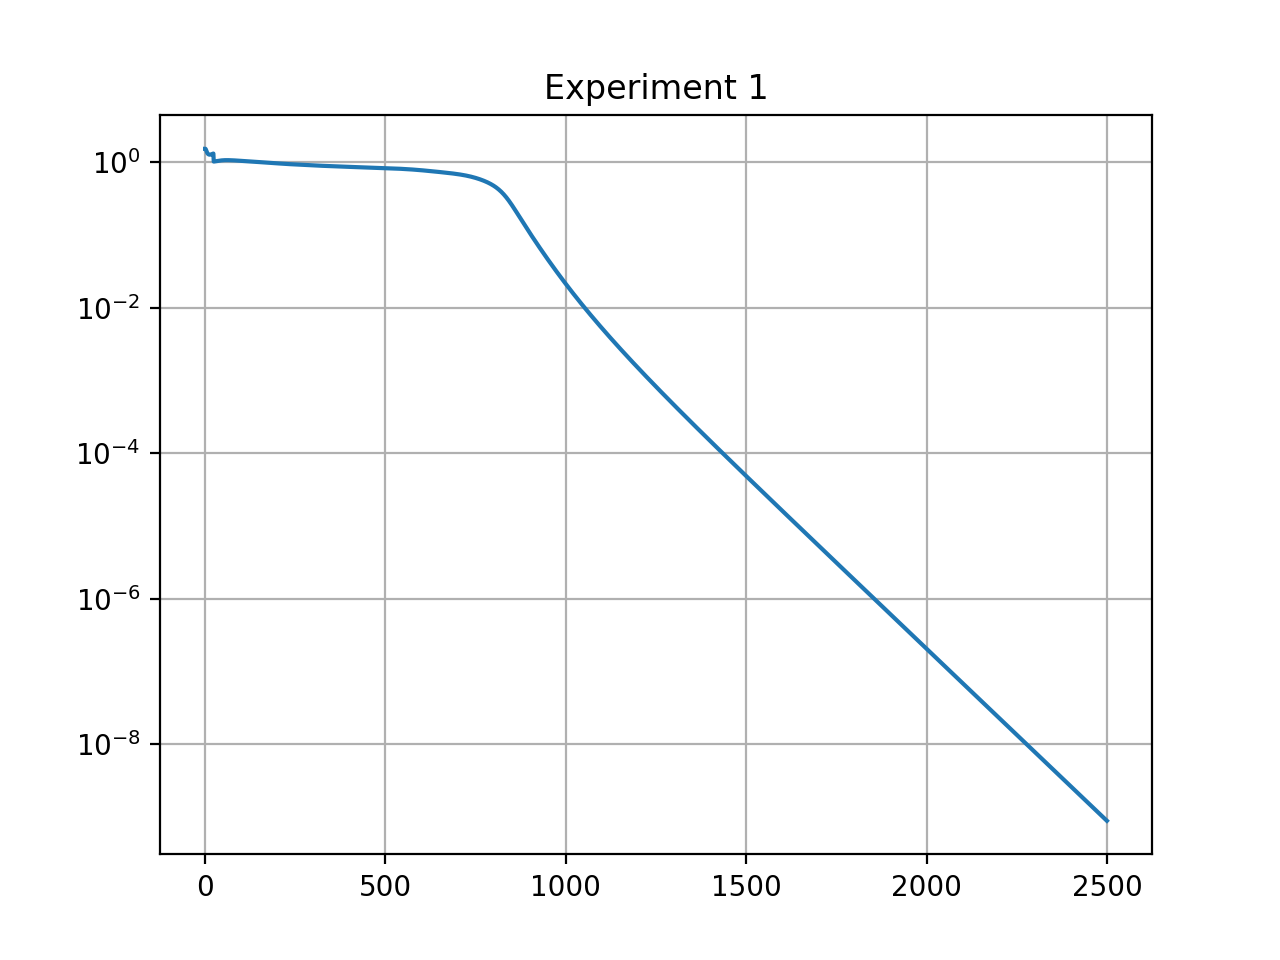
\includegraphics[width = 0.5\textwidth]{Figure_1.png}
  \caption{实验 1}
  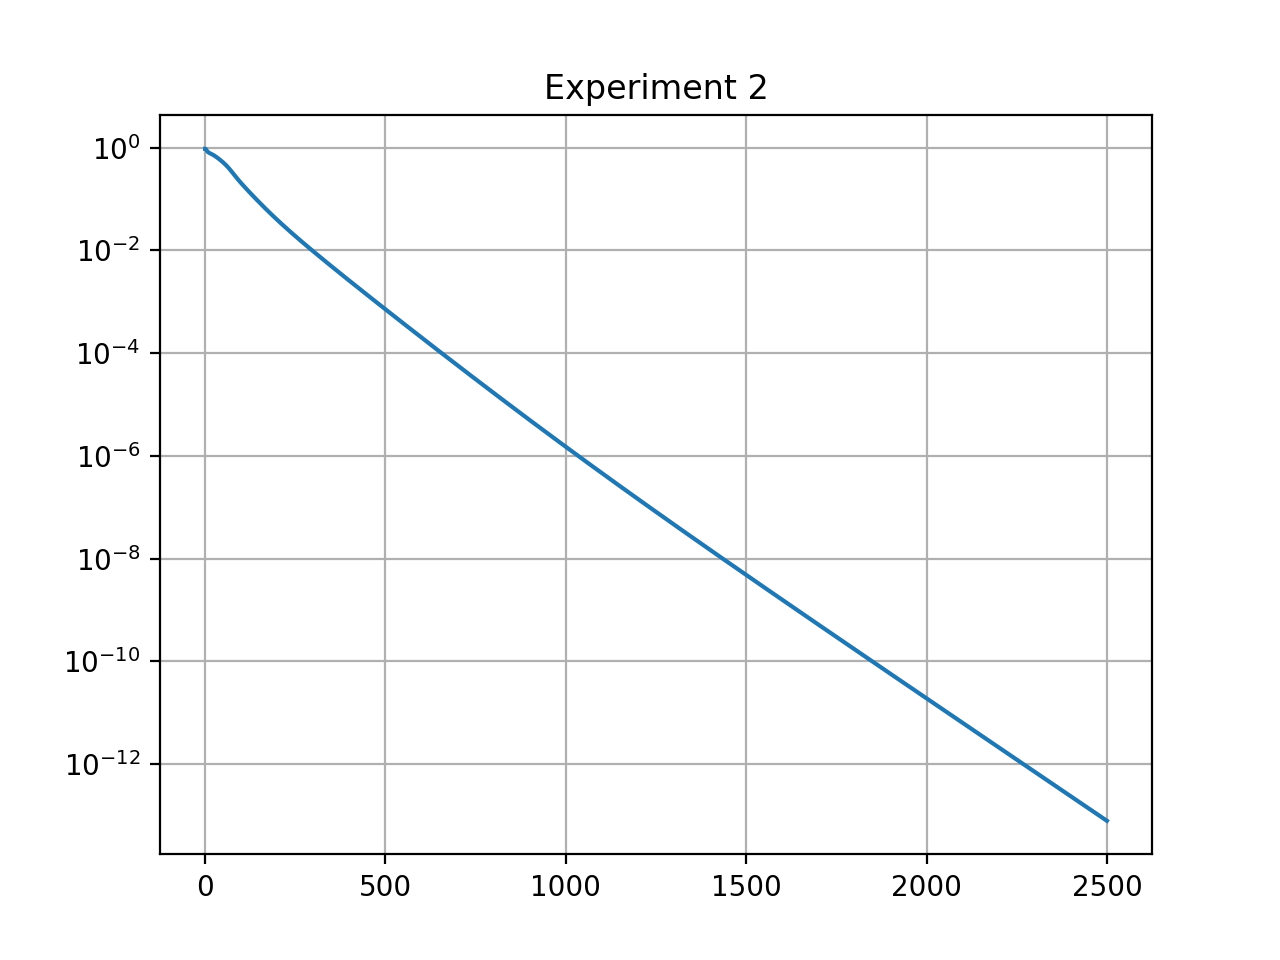
\includegraphics[width = 0.5\textwidth]{Figure_2.png}
  \caption{实验 2}
  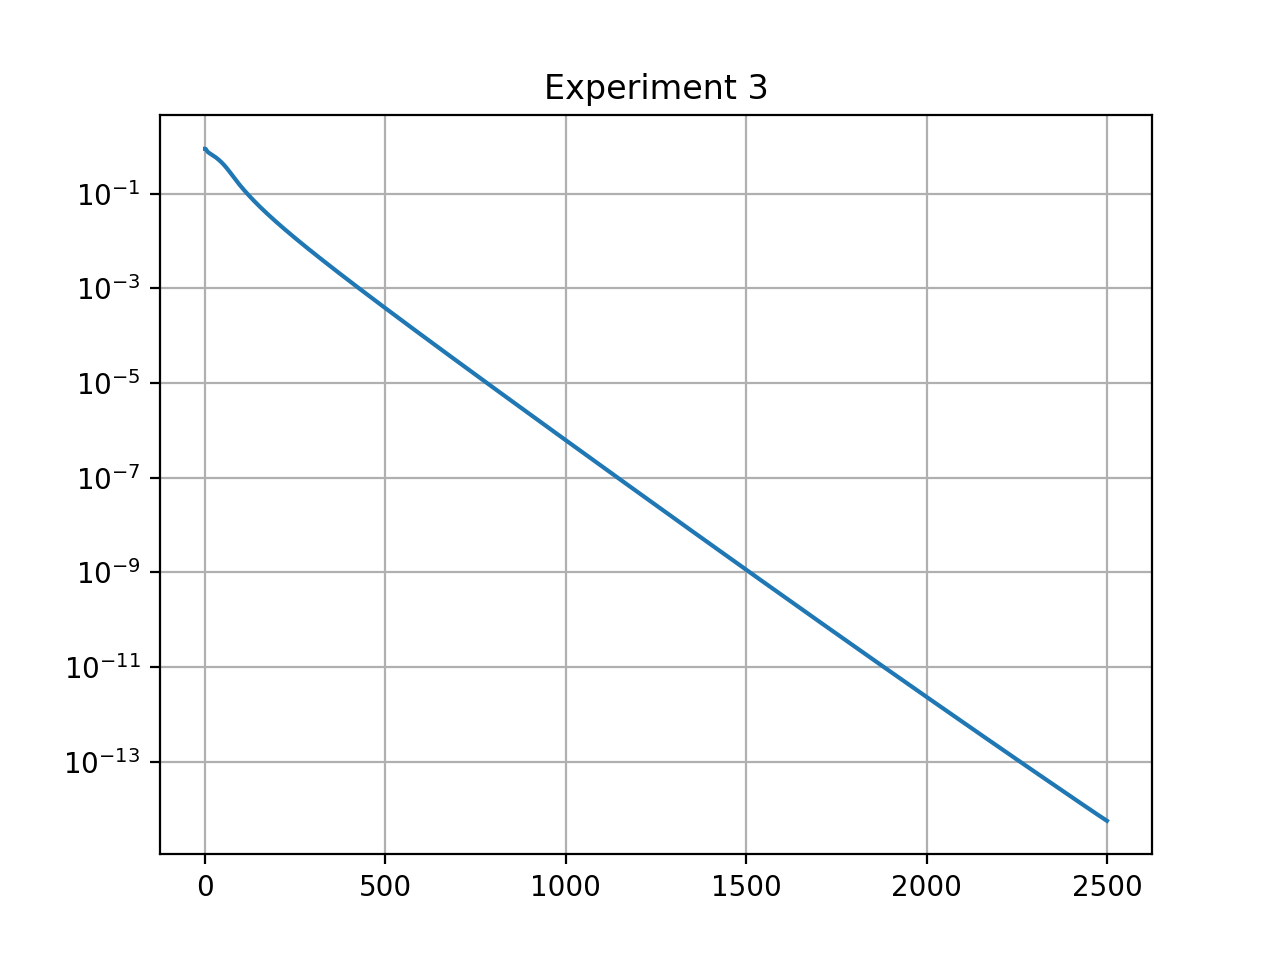
\includegraphics[width = 0.5\textwidth]{Figure_3.png}
  \caption{实验 3}
\end{figure}


\end{document}
